\documentclass[]{article}
\usepackage{lmodern}
\usepackage{amssymb,amsmath}
\usepackage{ifxetex,ifluatex}
\usepackage{fixltx2e} % provides \textsubscript
\ifnum 0\ifxetex 1\fi\ifluatex 1\fi=0 % if pdftex
  \usepackage[T1]{fontenc}
  \usepackage[utf8]{inputenc}
\else % if luatex or xelatex
  \ifxetex
    \usepackage{mathspec}
  \else
    \usepackage{fontspec}
  \fi
  \defaultfontfeatures{Ligatures=TeX,Scale=MatchLowercase}
\fi
% use upquote if available, for straight quotes in verbatim environments
\IfFileExists{upquote.sty}{\usepackage{upquote}}{}
% use microtype if available
\IfFileExists{microtype.sty}{%
\usepackage{microtype}
\UseMicrotypeSet[protrusion]{basicmath} % disable protrusion for tt fonts
}{}
\usepackage[margin=2.54cm]{geometry}
\usepackage{hyperref}
\hypersetup{unicode=true,
            pdftitle={Assignment 6: Time Series Analysis},
            pdfauthor={Jake Greif},
            pdfborder={0 0 0},
            breaklinks=true}
\urlstyle{same}  % don't use monospace font for urls
\usepackage{color}
\usepackage{fancyvrb}
\newcommand{\VerbBar}{|}
\newcommand{\VERB}{\Verb[commandchars=\\\{\}]}
\DefineVerbatimEnvironment{Highlighting}{Verbatim}{commandchars=\\\{\}}
% Add ',fontsize=\small' for more characters per line
\usepackage{framed}
\definecolor{shadecolor}{RGB}{248,248,248}
\newenvironment{Shaded}{\begin{snugshade}}{\end{snugshade}}
\newcommand{\AlertTok}[1]{\textcolor[rgb]{0.94,0.16,0.16}{#1}}
\newcommand{\AnnotationTok}[1]{\textcolor[rgb]{0.56,0.35,0.01}{\textbf{\textit{#1}}}}
\newcommand{\AttributeTok}[1]{\textcolor[rgb]{0.77,0.63,0.00}{#1}}
\newcommand{\BaseNTok}[1]{\textcolor[rgb]{0.00,0.00,0.81}{#1}}
\newcommand{\BuiltInTok}[1]{#1}
\newcommand{\CharTok}[1]{\textcolor[rgb]{0.31,0.60,0.02}{#1}}
\newcommand{\CommentTok}[1]{\textcolor[rgb]{0.56,0.35,0.01}{\textit{#1}}}
\newcommand{\CommentVarTok}[1]{\textcolor[rgb]{0.56,0.35,0.01}{\textbf{\textit{#1}}}}
\newcommand{\ConstantTok}[1]{\textcolor[rgb]{0.00,0.00,0.00}{#1}}
\newcommand{\ControlFlowTok}[1]{\textcolor[rgb]{0.13,0.29,0.53}{\textbf{#1}}}
\newcommand{\DataTypeTok}[1]{\textcolor[rgb]{0.13,0.29,0.53}{#1}}
\newcommand{\DecValTok}[1]{\textcolor[rgb]{0.00,0.00,0.81}{#1}}
\newcommand{\DocumentationTok}[1]{\textcolor[rgb]{0.56,0.35,0.01}{\textbf{\textit{#1}}}}
\newcommand{\ErrorTok}[1]{\textcolor[rgb]{0.64,0.00,0.00}{\textbf{#1}}}
\newcommand{\ExtensionTok}[1]{#1}
\newcommand{\FloatTok}[1]{\textcolor[rgb]{0.00,0.00,0.81}{#1}}
\newcommand{\FunctionTok}[1]{\textcolor[rgb]{0.00,0.00,0.00}{#1}}
\newcommand{\ImportTok}[1]{#1}
\newcommand{\InformationTok}[1]{\textcolor[rgb]{0.56,0.35,0.01}{\textbf{\textit{#1}}}}
\newcommand{\KeywordTok}[1]{\textcolor[rgb]{0.13,0.29,0.53}{\textbf{#1}}}
\newcommand{\NormalTok}[1]{#1}
\newcommand{\OperatorTok}[1]{\textcolor[rgb]{0.81,0.36,0.00}{\textbf{#1}}}
\newcommand{\OtherTok}[1]{\textcolor[rgb]{0.56,0.35,0.01}{#1}}
\newcommand{\PreprocessorTok}[1]{\textcolor[rgb]{0.56,0.35,0.01}{\textit{#1}}}
\newcommand{\RegionMarkerTok}[1]{#1}
\newcommand{\SpecialCharTok}[1]{\textcolor[rgb]{0.00,0.00,0.00}{#1}}
\newcommand{\SpecialStringTok}[1]{\textcolor[rgb]{0.31,0.60,0.02}{#1}}
\newcommand{\StringTok}[1]{\textcolor[rgb]{0.31,0.60,0.02}{#1}}
\newcommand{\VariableTok}[1]{\textcolor[rgb]{0.00,0.00,0.00}{#1}}
\newcommand{\VerbatimStringTok}[1]{\textcolor[rgb]{0.31,0.60,0.02}{#1}}
\newcommand{\WarningTok}[1]{\textcolor[rgb]{0.56,0.35,0.01}{\textbf{\textit{#1}}}}
\usepackage{graphicx,grffile}
\makeatletter
\def\maxwidth{\ifdim\Gin@nat@width>\linewidth\linewidth\else\Gin@nat@width\fi}
\def\maxheight{\ifdim\Gin@nat@height>\textheight\textheight\else\Gin@nat@height\fi}
\makeatother
% Scale images if necessary, so that they will not overflow the page
% margins by default, and it is still possible to overwrite the defaults
% using explicit options in \includegraphics[width, height, ...]{}
\setkeys{Gin}{width=\maxwidth,height=\maxheight,keepaspectratio}
\IfFileExists{parskip.sty}{%
\usepackage{parskip}
}{% else
\setlength{\parindent}{0pt}
\setlength{\parskip}{6pt plus 2pt minus 1pt}
}
\setlength{\emergencystretch}{3em}  % prevent overfull lines
\providecommand{\tightlist}{%
  \setlength{\itemsep}{0pt}\setlength{\parskip}{0pt}}
\setcounter{secnumdepth}{0}
% Redefines (sub)paragraphs to behave more like sections
\ifx\paragraph\undefined\else
\let\oldparagraph\paragraph
\renewcommand{\paragraph}[1]{\oldparagraph{#1}\mbox{}}
\fi
\ifx\subparagraph\undefined\else
\let\oldsubparagraph\subparagraph
\renewcommand{\subparagraph}[1]{\oldsubparagraph{#1}\mbox{}}
\fi

%%% Use protect on footnotes to avoid problems with footnotes in titles
\let\rmarkdownfootnote\footnote%
\def\footnote{\protect\rmarkdownfootnote}

%%% Change title format to be more compact
\usepackage{titling}

% Create subtitle command for use in maketitle
\providecommand{\subtitle}[1]{
  \posttitle{
    \begin{center}\large#1\end{center}
    }
}

\setlength{\droptitle}{-2em}

  \title{Assignment 6: Time Series Analysis}
    \pretitle{\vspace{\droptitle}\centering\huge}
  \posttitle{\par}
    \author{Jake Greif}
    \preauthor{\centering\large\emph}
  \postauthor{\par}
    \date{}
    \predate{}\postdate{}
  

\begin{document}
\maketitle

\hypertarget{overview}{%
\subsection{OVERVIEW}\label{overview}}

This exercise accompanies the lessons in Hydrologic Data Analysis on
time series analysis

\hypertarget{directions}{%
\subsection{Directions}\label{directions}}

\begin{enumerate}
\def\labelenumi{\arabic{enumi}.}
\tightlist
\item
  Change ``Student Name'' on line 3 (above) with your name.
\item
  Work through the steps, \textbf{creating code and output} that fulfill
  each instruction.
\item
  Be sure to \textbf{answer the questions} in this assignment document.
\item
  When you have completed the assignment, \textbf{Knit} the text and
  code into a single pdf file.
\item
  After Knitting, submit the completed exercise (pdf file) to the
  dropbox in Sakai. Add your last name into the file name (e.g.,
  ``A06\_Salk.html'') prior to submission.
\end{enumerate}

The completed exercise is due on 11 October 2019 at 9:00 am.

\hypertarget{setup}{%
\subsection{Setup}\label{setup}}

\begin{enumerate}
\def\labelenumi{\arabic{enumi}.}
\tightlist
\item
  Verify your working directory is set to the R project file,
\item
  Load the tidyverse, lubridate, trend, and dataRetrieval packages.
\item
  Set your ggplot theme (can be theme\_classic or something else)
\item
  Load the ClearCreekDischarge.Monthly.csv file from the processed data
  folder. Call this data frame ClearCreekDischarge.Monthly.
\end{enumerate}

\begin{Shaded}
\begin{Highlighting}[]
\KeywordTok{getwd}\NormalTok{()}
\end{Highlighting}
\end{Shaded}

\begin{verbatim}
## [1] "/Users/jakegreif/Duke/Fall_2019/Hydrologic_Data_Analysis"
\end{verbatim}

\begin{Shaded}
\begin{Highlighting}[]
\KeywordTok{library}\NormalTok{(tidyverse)}
\KeywordTok{library}\NormalTok{(lubridate)}
\KeywordTok{library}\NormalTok{(dataRetrieval)}
\KeywordTok{library}\NormalTok{(trend)}

\KeywordTok{theme_set}\NormalTok{(}\KeywordTok{theme_classic}\NormalTok{())}

\NormalTok{ClearCreekDischarge.Monthly <-}\StringTok{ }
\StringTok{  }\KeywordTok{read.csv}\NormalTok{(}\StringTok{"./Data/Processed/ClearCreekDischarge.Monthly.csv"}\NormalTok{)}
\end{Highlighting}
\end{Shaded}

\hypertarget{time-series-decomposition}{%
\subsection{Time Series Decomposition}\label{time-series-decomposition}}

\begin{enumerate}
\def\labelenumi{\arabic{enumi}.}
\setcounter{enumi}{4}
\tightlist
\item
  Create a new data frame that includes daily mean discharge at the Eno
  River for all available dates (\texttt{siteNumbers\ =\ "02085070"}).
  Rename the columns accordingly.
\item
  Plot discharge over time with geom\_line. Make sure axis labels are
  formatted appropriately.
\item
  Create a time series of discharge
\item
  Decompose the time series using the \texttt{stl} function.
\item
  Visualize the decomposed time series.
\end{enumerate}

\begin{Shaded}
\begin{Highlighting}[]
\CommentTok{# Import data}
\NormalTok{EnoDischarge <-}\StringTok{ }\KeywordTok{readNWISdv}\NormalTok{(}\DataTypeTok{siteNumbers =} \StringTok{"02085070"}\NormalTok{,}
                     \DataTypeTok{parameterCd =} \StringTok{"00060"}\NormalTok{, }
                     \DataTypeTok{startDate =} \StringTok{""}\NormalTok{,}
                     \DataTypeTok{endDate =} \StringTok{""}\NormalTok{)}
\KeywordTok{names}\NormalTok{(EnoDischarge)[}\DecValTok{4}\OperatorTok{:}\DecValTok{5}\NormalTok{] <-}\StringTok{ }\KeywordTok{c}\NormalTok{(}\StringTok{"Discharge"}\NormalTok{, }\StringTok{"Approval.Code"}\NormalTok{)}

\CommentTok{# Plot discharge over time}
\NormalTok{EnoPlot <-}\StringTok{ }
\StringTok{  }\KeywordTok{ggplot}\NormalTok{(EnoDischarge, }\KeywordTok{aes}\NormalTok{(}\DataTypeTok{x =}\NormalTok{ Date, }\DataTypeTok{y =}\NormalTok{ Discharge)) }\OperatorTok{+}
\StringTok{  }\KeywordTok{geom_line}\NormalTok{() }\OperatorTok{+}
\StringTok{  }\KeywordTok{labs}\NormalTok{(}\DataTypeTok{x =} \StringTok{""}\NormalTok{, }\DataTypeTok{y =} \KeywordTok{expression}\NormalTok{(}\StringTok{"Discharge (ft"}\OperatorTok{^}\DecValTok{3}\OperatorTok{*}\StringTok{"/s)"}\NormalTok{))}
\KeywordTok{print}\NormalTok{(EnoPlot)}
\end{Highlighting}
\end{Shaded}

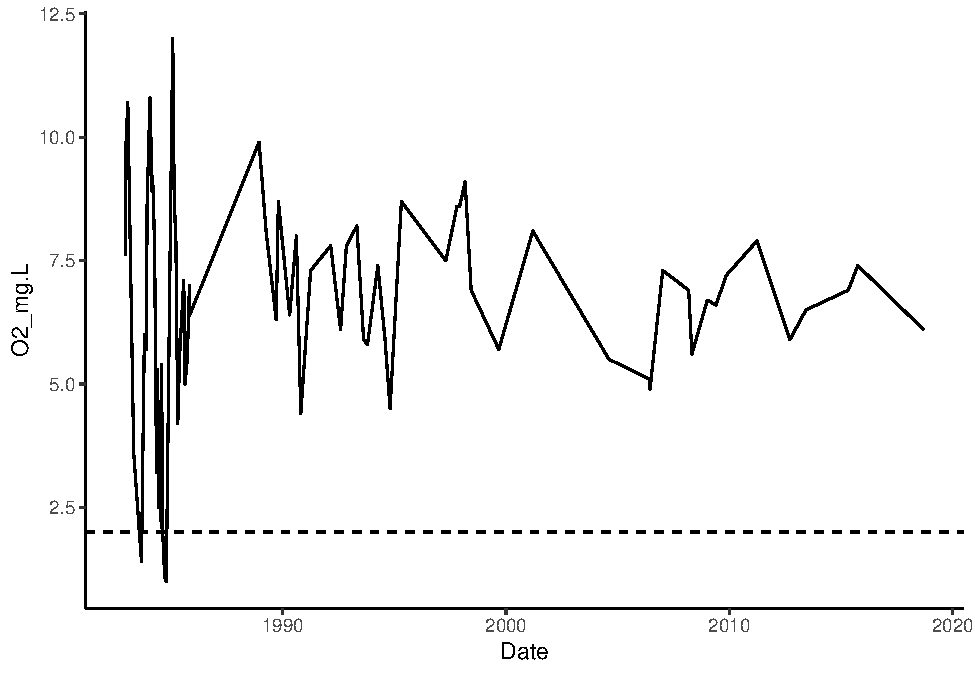
\includegraphics{A06_TimeSeries_files/figure-latex/unnamed-chunk-1-1.pdf}

\begin{Shaded}
\begin{Highlighting}[]
\CommentTok{# Creat time series}
\NormalTok{Eno_ts <-}\StringTok{ }\KeywordTok{ts}\NormalTok{(EnoDischarge[[}\DecValTok{4}\NormalTok{]], }\DataTypeTok{frequency =} \DecValTok{365}\NormalTok{)}

\CommentTok{# Decompose time series}
\NormalTok{Eno_Decomposed <-}\StringTok{ }\KeywordTok{stl}\NormalTok{(Eno_ts, }\DataTypeTok{s.window =} \StringTok{"periodic"}\NormalTok{)}

\CommentTok{# Visualize the decomposed series. }
\KeywordTok{plot}\NormalTok{(Eno_Decomposed)}
\end{Highlighting}
\end{Shaded}

\includegraphics{A06_TimeSeries_files/figure-latex/unnamed-chunk-1-2.pdf}

\begin{enumerate}
\def\labelenumi{\arabic{enumi}.}
\setcounter{enumi}{9}
\tightlist
\item
  How do the seasonal and trend components of the decomposition compare
  to the Clear Creek discharge dataset? Are they similar in magnitude?
\end{enumerate}

\begin{quote}
Seasonal: The seasonal component of the Eno is noisier and lesser in
magnitude compared to Clear Creek.
\end{quote}

\begin{quote}
Trend: The trend component of the Eno is lower in magnitude compared to
Clear Creek, but Clear Creek trend seems to be more smooth (less intense
changes) than the Eno.
\end{quote}

\hypertarget{trend-analysis}{%
\subsection{Trend Analysis}\label{trend-analysis}}

Research question: Has there been a monotonic trend in discharge in
Clear Creek over the period of study?

\begin{enumerate}
\def\labelenumi{\arabic{enumi}.}
\setcounter{enumi}{10}
\tightlist
\item
  Generate a time series of monthly discharge in Clear Creek from the
  ClearCreekDischarge.Monthly data frame. This time series should
  include just one column (discharge).
\item
  Run a Seasonal Mann-Kendall test on the monthly discharge data.
  Inspect the overall trend and the monthly trends.
\end{enumerate}

\begin{Shaded}
\begin{Highlighting}[]
\CommentTok{# Plot, observe data}
\NormalTok{ClearCreekDischarge <-}\StringTok{ }\KeywordTok{readNWISdv}\NormalTok{(}\DataTypeTok{siteNumbers =} \StringTok{"06719505"}\NormalTok{,}
                     \DataTypeTok{parameterCd =} \StringTok{"00060"}\NormalTok{, }\CommentTok{# discharge (ft3/s)}
                     \DataTypeTok{startDate =} \StringTok{""}\NormalTok{,}
                     \DataTypeTok{endDate =} \StringTok{""}\NormalTok{)}
\KeywordTok{names}\NormalTok{(ClearCreekDischarge)[}\DecValTok{4}\OperatorTok{:}\DecValTok{5}\NormalTok{] <-}\StringTok{ }\KeywordTok{c}\NormalTok{(}\StringTok{"Discharge"}\NormalTok{, }\StringTok{"Approval.Code"}\NormalTok{)}

\KeywordTok{ggplot}\NormalTok{(ClearCreekDischarge, }\KeywordTok{aes}\NormalTok{(}\DataTypeTok{x =}\NormalTok{ Date, }\DataTypeTok{y =}\NormalTok{ Discharge)) }\OperatorTok{+}
\StringTok{  }\KeywordTok{geom_point}\NormalTok{()}
\end{Highlighting}
\end{Shaded}

\includegraphics{A06_TimeSeries_files/figure-latex/unnamed-chunk-2-1.pdf}

\begin{Shaded}
\begin{Highlighting}[]
\CommentTok{# Generate time series}
\NormalTok{ClearCreek_ts <-}\StringTok{ }\KeywordTok{ts}\NormalTok{(ClearCreekDischarge.Monthly[[}\DecValTok{3}\NormalTok{]], }\DataTypeTok{frequency =} \DecValTok{12}\NormalTok{)}

\CommentTok{# Run SMK test}
\NormalTok{CCtrend <-}\StringTok{ }\KeywordTok{smk.test}\NormalTok{(ClearCreek_ts)}

\CommentTok{# Inspect results}
\NormalTok{CCtrend}
\end{Highlighting}
\end{Shaded}

\begin{verbatim}
## 
##  Seasonal Mann-Kendall trend test (Hirsch-Slack test)
## 
## data:  ClearCreek_ts
## z = 1.6586, p-value = 0.09719
## alternative hypothesis: true S is not equal to 0
## sample estimates:
##      S   varS 
##    590 126102
\end{verbatim}

\begin{Shaded}
\begin{Highlighting}[]
\KeywordTok{summary}\NormalTok{(CCtrend)}
\end{Highlighting}
\end{Shaded}

\begin{verbatim}
## 
##  Seasonal Mann-Kendall trend test (Hirsch-Slack test)
## 
## data: ClearCreek_ts
## alternative hypothesis: two.sided
## 
## Statistics for individual seasons
## 
## H0
##                      S  varS    tau      z Pr(>|z|)  
## Season 1:   S = 0   64 11154  0.062  0.597 0.550828  
## Season 2:   S = 0   24 10450  0.024  0.225 0.821984  
## Season 3:   S = 0   30 10450  0.030  0.284 0.776650  
## Season 4:   S = 0   35 10449  0.035  0.333 0.739425  
## Season 5:   S = 0    4 10450  0.004  0.029 0.976588  
## Season 6:   S = 0  204 10450  0.206  1.986 0.047054 *
## Season 7:   S = 0  230 10450  0.232  2.240 0.025081 *
## Season 8:   S = 0  148 10450  0.149  1.438 0.150434  
## Season 9:   S = 0   94 10450  0.095  0.910 0.362951  
## Season 10:   S = 0 -54 10450 -0.055 -0.518 0.604135  
## Season 11:   S = 0 -99 10449 -0.100 -0.959 0.337703  
## Season 12:   S = 0 -90 10450 -0.091 -0.871 0.383958  
## ---
## Signif. codes:  0 '***' 0.001 '**' 0.01 '*' 0.05 '.' 0.1 ' ' 1
\end{verbatim}

\begin{enumerate}
\def\labelenumi{\arabic{enumi}.}
\setcounter{enumi}{12}
\tightlist
\item
  Is there an overall monotonic trend in discharge over time? If so, is
  it positive or negative?
\end{enumerate}

\begin{quote}
There is not a significant overall monotonic trend in discharge over
time.
\end{quote}

\begin{enumerate}
\def\labelenumi{\arabic{enumi}.}
\setcounter{enumi}{13}
\tightlist
\item
  Are there any monthly monotonic trends in discharge over time? If so,
  during which months do they occur and are they positive or negative?
\end{enumerate}

\begin{quote}
There are posotive monotonic trends in discharge in the months of June
and July.
\end{quote}

\hypertarget{reflection}{%
\subsection{Reflection}\label{reflection}}

\begin{enumerate}
\def\labelenumi{\arabic{enumi}.}
\setcounter{enumi}{14}
\tightlist
\item
  What are 2-3 conclusions or summary points about time series you
  learned through your analysis?
\end{enumerate}

\begin{quote}
Time series contain a lot of useful information, but they require high
quality data. It is possible to run trend analyses in the abscence of
high quality data, but it's important to carefully choose the proper
interpolation techniques and trend analyses because certain types of
statistical tests are only appropriate for specific types of data.
\end{quote}

\begin{enumerate}
\def\labelenumi{\arabic{enumi}.}
\setcounter{enumi}{15}
\tightlist
\item
  What data, visualizations, and/or models supported your conclusions
  from 12?
\end{enumerate}

\begin{quote}
The assumptions for each of the monotonic trend tests are all slightly
different and require careful consideration of the data before using
them. The `challenges' of time series analysis layed out at the
beginning of lesson 11 also highlight the difficulty of analyzing time
series.
\end{quote}

\begin{enumerate}
\def\labelenumi{\arabic{enumi}.}
\setcounter{enumi}{16}
\tightlist
\item
  Did hands-on data analysis impact your learning about time series
  relative to a theory-based lesson? If so, how?
\end{enumerate}

\begin{quote}
Yes, because the hands-on data analysis allowed me to see how the
statistical tests can be applied. Without the hands-on experience, I
would have a much more difficult time understanding how to apply the
statistical tests to data in the future.
\end{quote}

\begin{enumerate}
\def\labelenumi{\arabic{enumi}.}
\setcounter{enumi}{17}
\tightlist
\item
  How did the real-world data compare with your expectations from
  theory?
\end{enumerate}

\begin{quote}
I assumed that there would be more significant trends in discharge over
time or from month to month based on what I've learned about the impacts
of climate change on the hydrologic cycle.
\end{quote}


\end{document}
